  \documentclass{beamer}
\usepackage[utf8]{inputenc}
\usepackage{hyperref}
\usepackage{graphicx}

\usepackage{listings}
\lstset{frame=single,backgroundcolor=\color{lightgray}}
\usetheme{Warsaw}

  \title{Introduction to Linux}
  \author{Pierre Lindenbaum\\@yokofakun\\http://plindenbaum.blogspot.com}\institute{Institut du Thorax. Nantes. France}

\begin{document}

\begin{frame}
\titlepage
\end{frame}



\begin{frame}
\begin{figure}
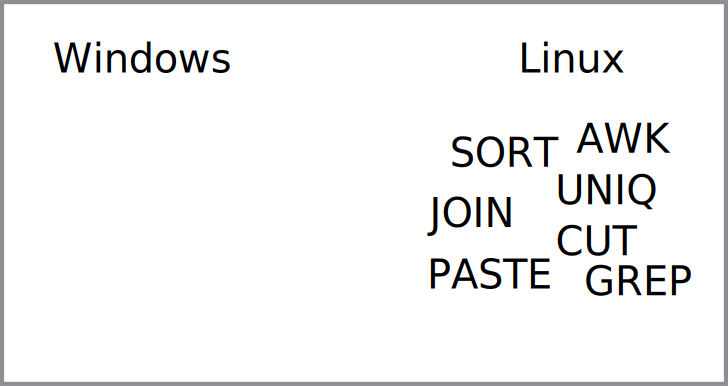
\includegraphics[scale=.5]{linux01.ps}
\end{figure}
\end{frame}

\begin{frame}
\begin{figure}
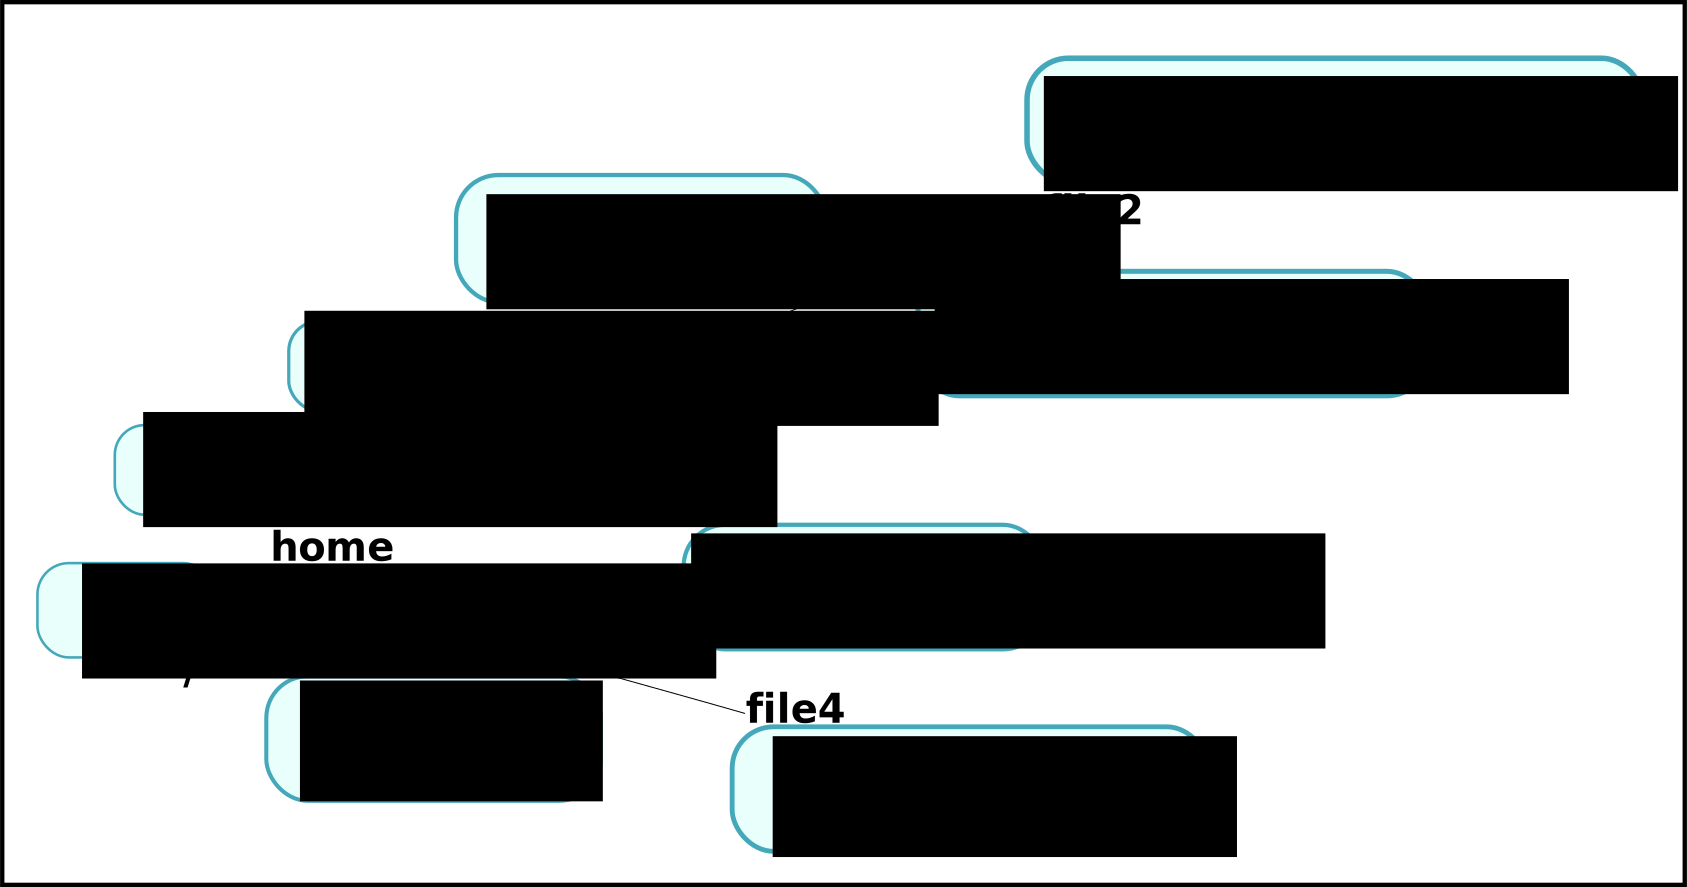
\includegraphics[scale=.23]{linux02.ps}
\end{figure}
\end{frame}

\begin{frame}
\begin{figure}
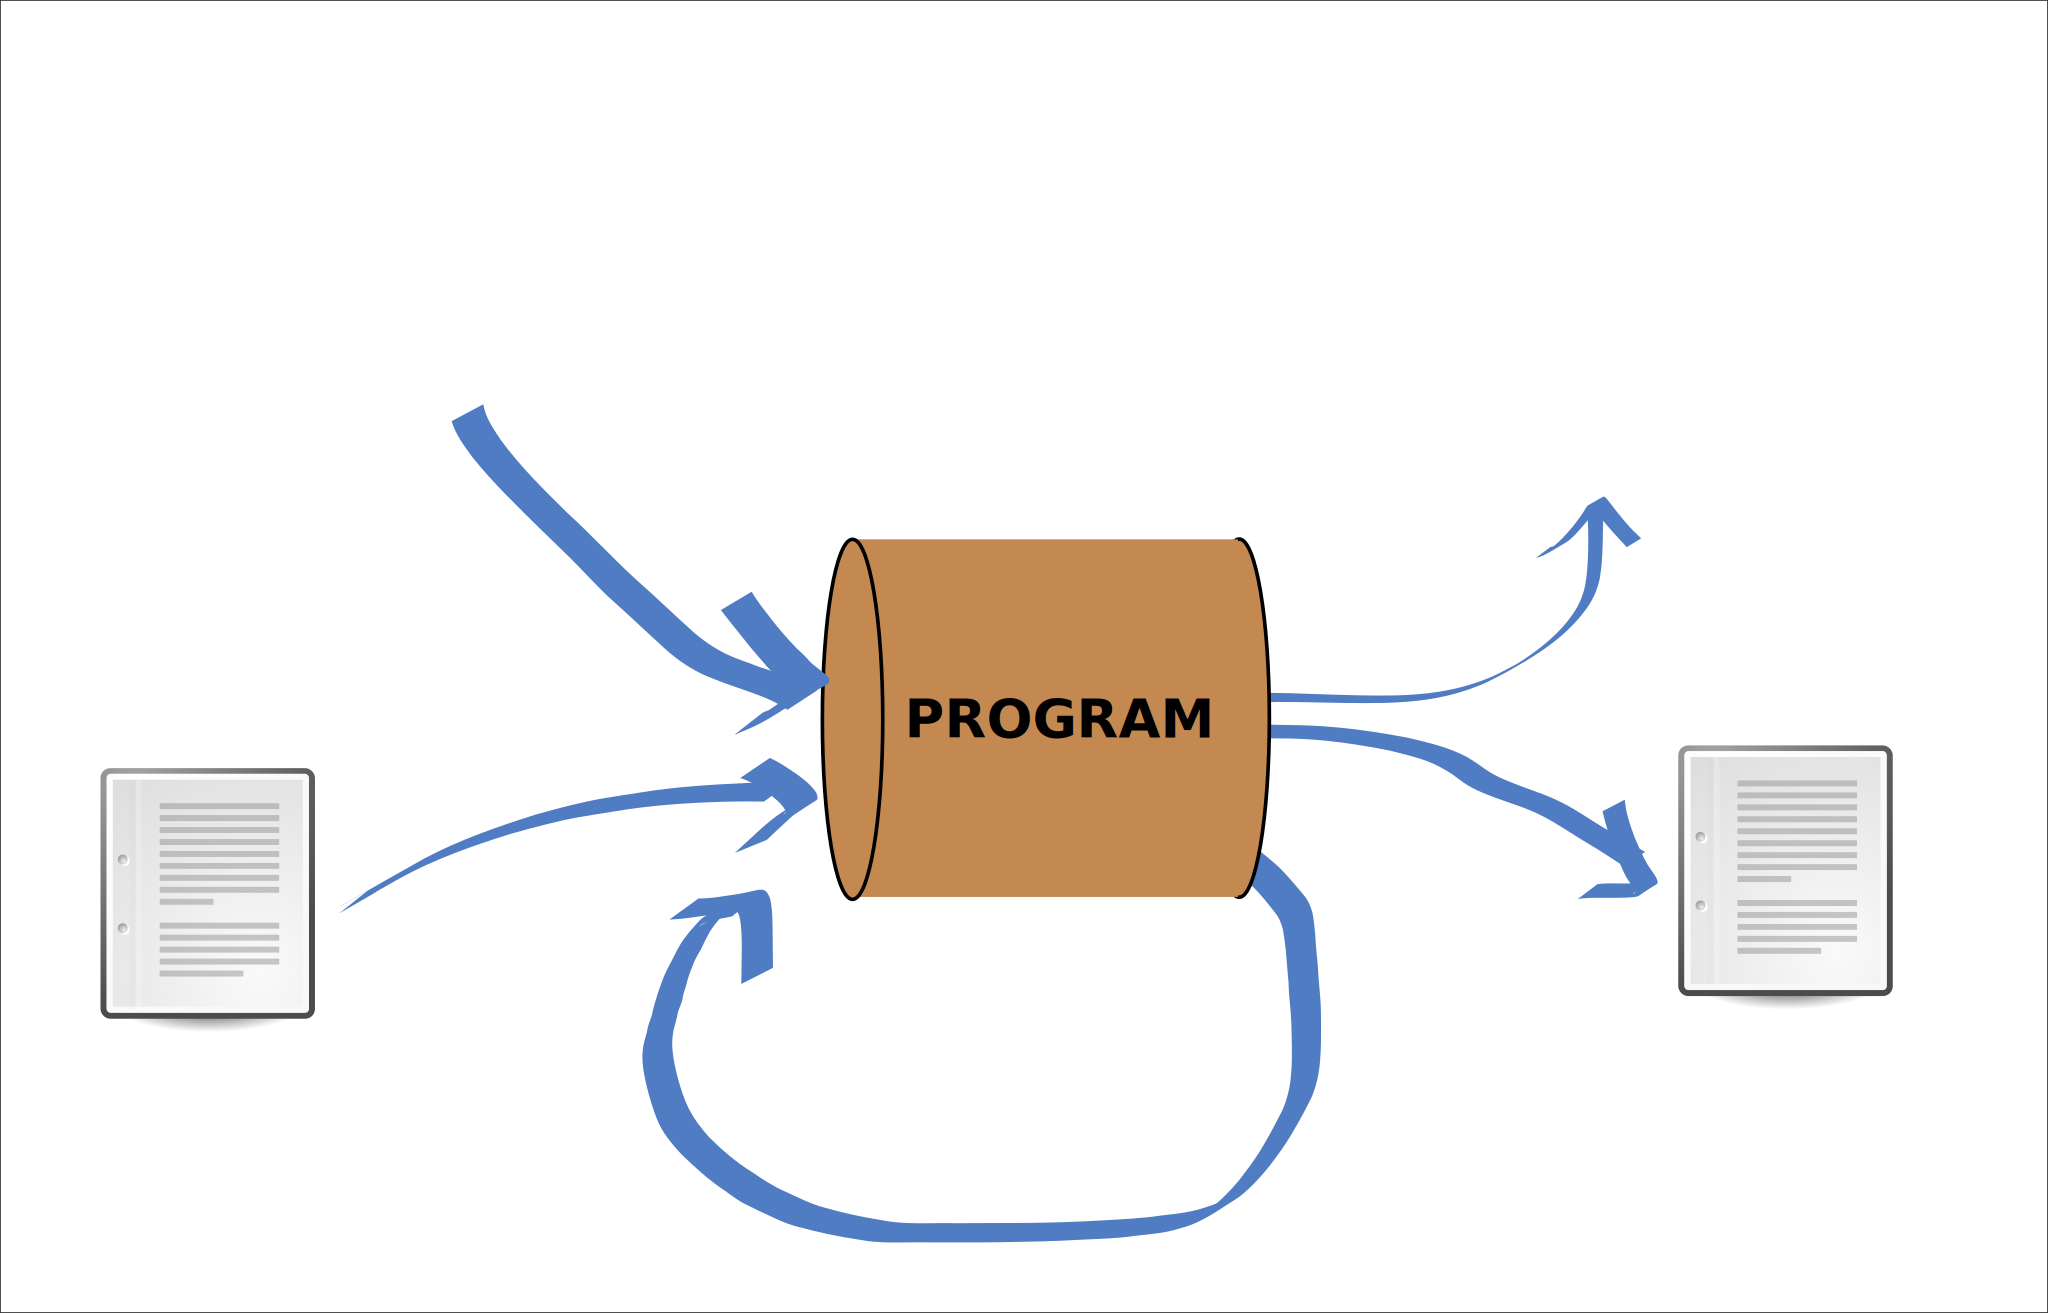
\includegraphics[scale=.15]{linux03.ps}
\end{figure}
\end{frame}


\begin{frame}[fragile]
\frametitle{Navigation}

where am I ?
\begin{lstlisting}[language=bash]
$ pwd
\end{lstlisting}

Go to directory dir1
\begin{lstlisting}[language=bash]
$ cd dir1
\end{lstlisting}

Go to directory dir1/dir2
\begin{lstlisting}[language=bash]
$ cd dir1/dir2
\end{lstlisting}


Go upper directory
\begin{lstlisting}[language=bash]
$ cd ..
\end{lstlisting}

Go upper directory and then go to dir4
\begin{lstlisting}[language=bash]
$ cd ../dir4
\end{lstlisting}


\end{frame}

\begin{frame}[fragile]
\frametitle{Navigation}

Go to the root
\begin{lstlisting}[language=bash]
$ cd /
\end{lstlisting}

Go to my home
\begin{lstlisting}[language=bash]
$ cd ~
\end{lstlisting}

Go to my previous directory
\begin{lstlisting}[language=bash]
$ cd /
\end{lstlisting}

\end{frame}

\begin{frame}[fragile]
 \begin{center}
    \huge{CASE matters}\\
    \end{center}
\begin{lstlisting}[language=bash]
$ cd dir1
\end{lstlisting}


\begin{lstlisting}[language=bash]
$ cd DIR1
\end{lstlisting}

\end{frame}


\begin{frame}[fragile]
 \begin{center}
    \huge{whitespaces matter}\\
    \end{center}
\begin{lstlisting}[language=bash]
$ cd my results
bash: cd: my: No such file or directory
\end{lstlisting}


\begin{lstlisting}[language=bash]
$ cd  "my results"
\end{lstlisting}

\begin{lstlisting}[language=bash]
$ cd my\ results
\end{lstlisting}
  
\end{frame}




\end{document}

